\section{Descrizione singoli componenti}

\subsection{Package \client{}}

\begin{figure}[H] \centering 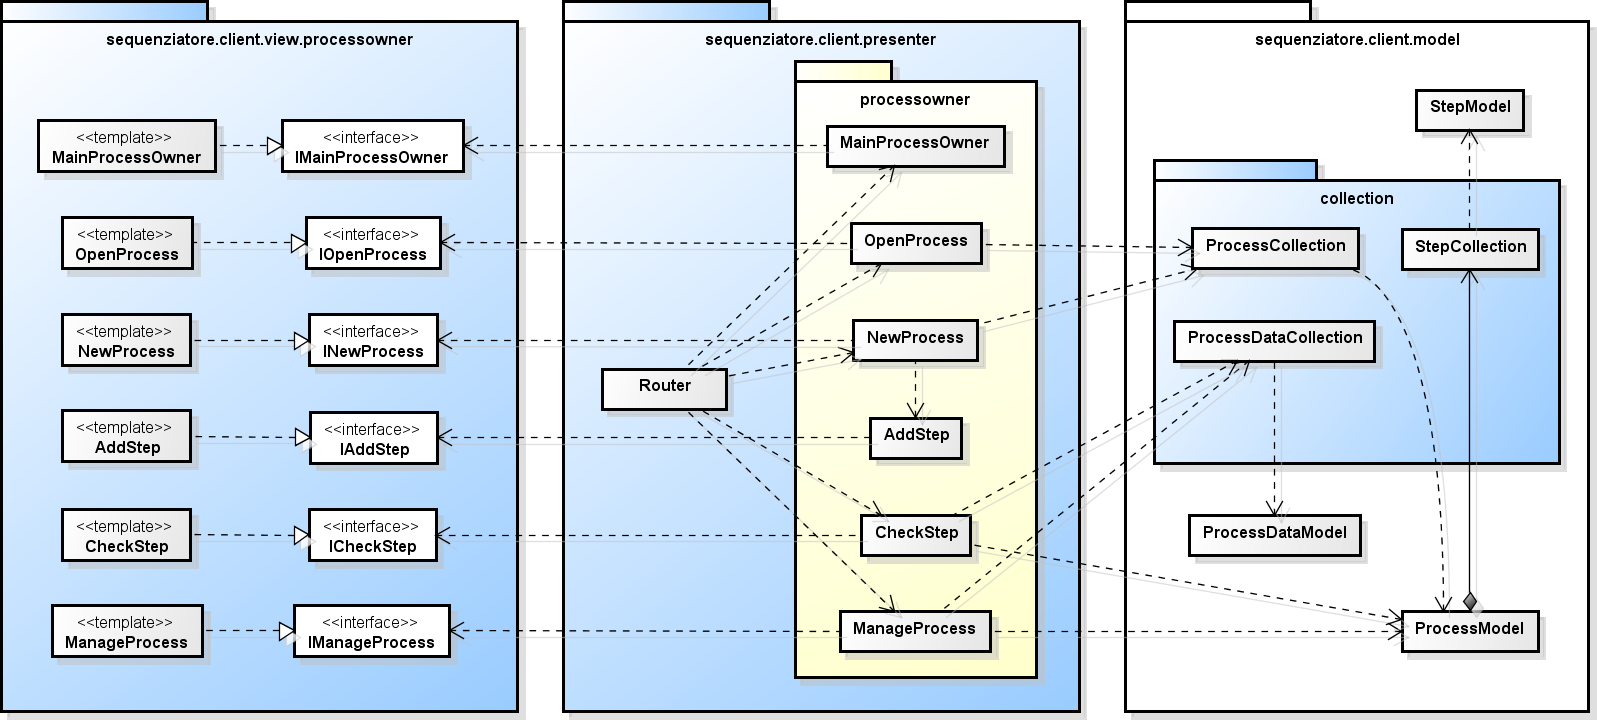
\includegraphics[width=%
\textwidth]
{./pack/POPackage.png} \caption{Diagramma componenti - \textit{process owner}}
\end{figure}

\begin{figure}[H] \centering 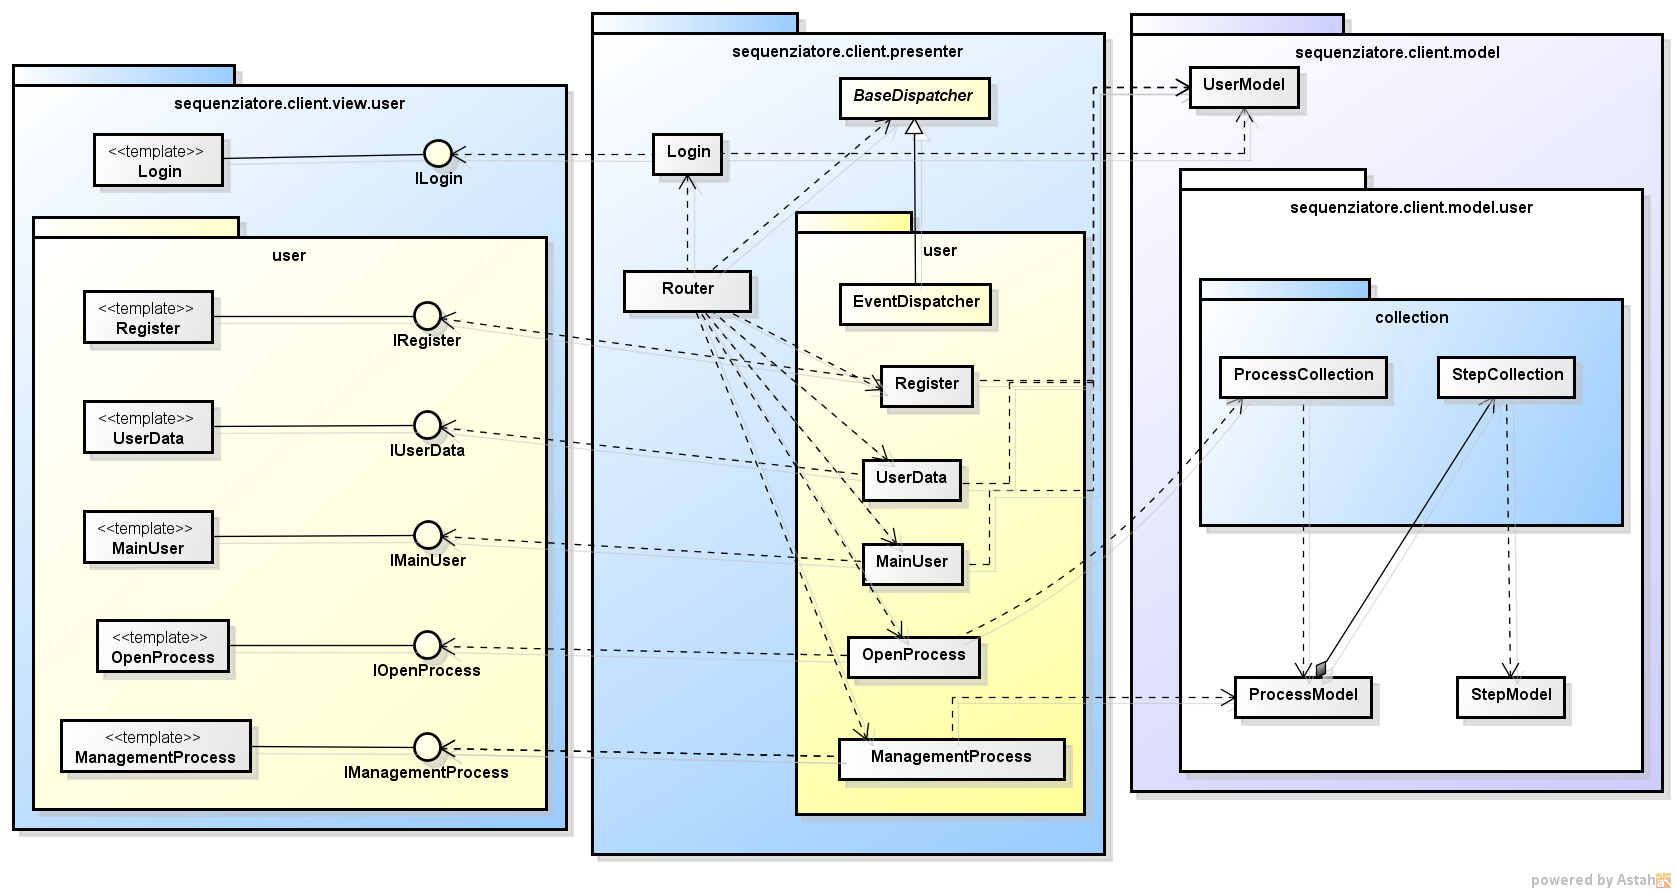
\includegraphics[width=%
\textwidth]
{./pack/UserMainPackage.png} \caption{Diagramma componenti - \textit{user}}
\end{figure}

\begin{figure}[H] \centering 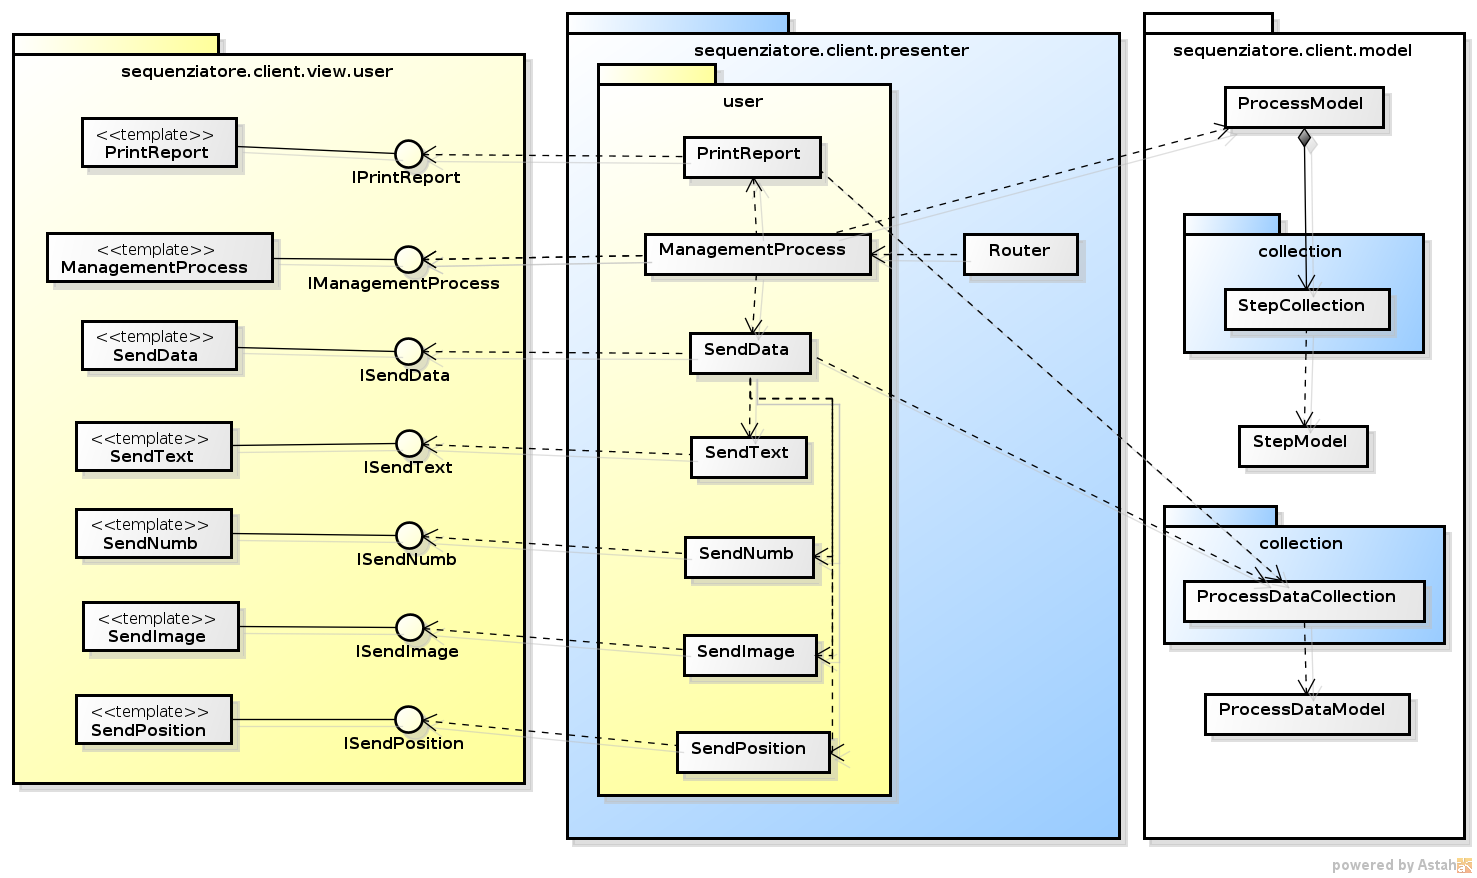
\includegraphics[width=%
\textwidth]
{./pack/ManageProcess.png} \caption{Diagramma componenti bis - \textit{user}}
\end{figure}


\subsection{Package \view{}}

\begin{figure}[H]
\centering
\includegraphics[trim=0cm 0.8cm 0cm 0cm,clip=true,scale=0.75]%
{./pack/UserViewA.png} \caption{Diagramma principale \textit{view} utente}
\end{figure}

\paragraph{ILogin}
\begin{itemize}
\item \textbf{Nome:} \texttt{ILogin};
\item \textbf{Package:} \texttt{\view{}};
\item \textbf{Descrizione:} Interfaccia che permette di gestire l'interfaccia grafica relativa alle richieste di autenticazione al sistema.
\end{itemize}

\paragraph{Login}
\begin{flushleft}
\begin{itemize}
\item \textbf{Nome:} \texttt{Login};
\item \textbf{Package:} \texttt{\view{}};
\item \textbf{Descrizione:} Componente che permette di gestire l'interfaccia grafica relativa alle richieste di autenticazione al sistema;
\item \textbf{Relazioni con altri componenti:}
\begin{sloppypar}
Il componente implementa l'interfaccia \texttt{\view{}.I\fshyp{}Lo\fshyp{}gin}.
\end{sloppypar}
\end{itemize}
\end{flushleft}

\subsubsection{Package sequenziatore.client.view.user}

\paragraph{IMainUser}
\begin{itemize}
\item \textbf{Nome:} \texttt{IMainUser};
\item \textbf{Descrizione:} Interfaccia che permette la gestione delle principali componenti dell'Interfaccia grafica dell'utente.
\end{itemize}

\paragraph{MainUser}
\begin{flushleft}
\begin{itemize}
\item \textbf{Nome:} \texttt{MainUser};
\item \textbf{Descrizione:} Classe che permette la gestione delle principali componenti dell'interfaccia grafica dell'utente;
\item \textbf{Relazioni con altri componenti:
\begin{sloppypar}
La classe implementa l'interfaccia \texttt{I\fshyp{}Main\fshyp{}U\fshyp{}ser}.
\end{sloppypar}
\end{itemize}
\end{flushleft}

\paragraph{ILogin}
\begin{itemize}
\item \textbf{Nome:} \texttt{ILogin};
\item \textbf{Descrizione:} Interfaccia che permette di gestire l'interfaccia grafica relativa alle richieste di autenticazione e chiusura della sessione da parte dell'utente.
\end{itemize}

\paragraph{Login}
\begin{flushleft}
\begin{itemize}
\item \textbf{Nome:} \texttt{Login};
\item \textbf{Descrizione:} Classe che permette di gestire dell'interfaccia grafica relativa alle richieste di autenticazione e chiusura della sessione da parte dell'utente;
\item \textbf{Relazioni con altri componenti:}
\begin{sloppypar}
La classe implementa l'interfaccia \texttt{I\fshyp{}Lo\fshyp{}gin}.
\end{sloppypar}
\end{itemize}
\end{flushleft}

\paragraph{IRegister}
\begin{itemize}
\item \textbf{Nome:} \texttt{IRegister};
\item \textbf{Package:} \texttt{\iViewUser{}};
\item \textbf{Descrizione:} Interfaccia che permette di gestire l'interfaccia grafica relativa alle richieste di registrazione da parte dell'utente.
\end{itemize}

\paragraph{Register}
\begin{flushleft}
\begin{itemize}
\item \textbf{Nome:} \texttt{Register};
\item \textbf{Descrizione:} Classe che permette di gestire dell'interfaccia grafica relativa alle richieste di registrazione da parte dell'utente;
\item \textbf{Relazioni con altri componenti:}
\begin{sloppypar}
La classe implementa l'interfaccia \texttt{I\fshyp{}Re\fshyp{}gis\fshyp{}ter}.
\end{sloppypar}
\end{itemize}
\end{flushleft}

\paragraph{IUserData}
\begin{itemize}
\item \textbf{Nome:} \texttt{IUserData};
\item \textbf{Descrizione:} Interfaccia che permette la realizzazione dei \textit{widget} per la visualizzazione dei dati dell'utente e la relativa modifica dei dati, dove possibile.
\end{itemize}

\paragraph{UserData}
\begin{flushleft}
\begin{itemize}
\item \textbf{Nome:} \texttt{UserData};
\item \textbf{Descrizione:} Classe che permette la realizzazione dei \textit{widget} che consentono visualizzazione e modifica dei dati dell'utente;
\item \textbf{Relazioni con altri componenti:}
\begin{sloppypar}
La classe implementa l'interfaccia \texttt{I\fshyp{}User\fshyp{}Da\fshyp{}ta}.
\end{sloppypar}
\end{itemize}
\end{flushleft}

\paragraph{IOpenProcess}
\begin{itemize}
\item \textbf{Nome:} \texttt{IOpenProcess};
\item \textbf{Descrizione:} Interfaccia che permette di realizzare i \textit{widget} per consentire la ricerca e la selezione di processi.
\end{itemize}

\paragraph{OpenProcess}
\begin{flushleft}
\begin{itemize}
\item \textbf{Nome:} \texttt{OpenProcess};
\item \textbf{Descrizione:} Classe che permette di realizzare i \textit{widget} per consentire l'apertura di un processo tramite ricerca o selezionandolo da una lista;
\item \textbf{Relazioni con altri componenti:}
\begin{sloppypar}
La classe implementa l'interfaccia \texttt{I\fshyp{}O\fshyp{}pen\fshyp{}Pro\fshyp{}cess}.
\end{sloppypar}
\end{itemize}
\end{flushleft}

\paragraph{IManagementProcess}
\begin{itemize}
\item \textbf{Nome:} \texttt{IManagementSelectedProcess};
\item \textbf{Descrizione:} Interfaccia che permette di realizzare i \textit{widget} per visualizzare lo stato corrente del processo selezionato e i vincoli per concludere il passo.
\end{itemize}

\paragraph{ManagementProcess}
\begin{flushleft}
\begin{itemize}
\item \textbf{Nome:} \texttt{ManagementProcess};
\item \textbf{Descrizione:} Classe che permette di realizzare i \textit{widget} per consentire la visualizzazione dello stato del processo selezionato e i vincoli per concludere il passo in corso;
\item \textbf{Relazioni con altri componenti:}
\begin{sloppypar}
La classe implementa l'interfaccia \texttt{I\fshyp{}Ma\fshyp{}na\fshyp{}ge\fshyp{}ment\fshyp{}Pro\fshyp{}cess}.
\end{sloppypar}
\end{itemize}
\end{flushleft}

\paragraph{ISendData}
\begin{itemize}
\item \textbf{Nome:} \texttt{ISendData};
\item \textbf{Descrizione:} Interfaccia che permette di realizzare i \textit{widget} per inviare i dati richiesti per la conclusione del passo.
\end{itemize}

\paragraph{SendData}
\begin{flushleft}
\begin{itemize}
\item \textbf{Nome:} \texttt{SendData};
\item \textbf{Descrizione:} Classe che permette di realizzare i \textit{widget} per consentire l'invio dei dati richiesti per la conclusione del passo in esecuzione;
\item \textbf{Relazioni con altri componenti:}
\begin{sloppypar}
La classe implementa l'interfaccia \texttt{\iViewUser{}::I\fshyp{}Send\fshyp{}Da\fshyp{}ta}.
\end{sloppypar}
\end{itemize}
\end{flushleft}

\paragraph{ISendText}
\begin{itemize}
\item \textbf{Nome:} \texttt{ISendData};
\item \textbf{Descrizione:} Interfaccia che permette di realizzare i \textit{widget} per inserire il testo da inviare per concludere il passo.
\end{itemize}

\paragraph{SendText}
\begin{flushleft}
\begin{itemize}
\item \textbf{Nome:} \texttt{SendData};
\item \textbf{Descrizione:} Classe che permette di realizzare i \textit{widget} che consentono di inserire il testo da inviare per concludere il passo in esecuzione;
\item \textbf{Relazioni con altri componenti:}
\begin{sloppypar}
La classe implementa l'interfaccia \texttt{\iViewUser{}::I\fshyp{}Send\fshyp{}Text}.
\end{sloppypar}
\end{itemize}
\end{flushleft}

\paragraph{ISendNumb}
\begin{itemize}
\item \textbf{Nome:} \texttt{ISendNumb};
\item \textbf{Descrizione:} Interfaccia che permette di realizzare i \textit{widget} per inserire i dati numerici da inviare per concludere il passo.
\end{itemize}

\paragraph{SendNumb}
\begin{flushleft}
\begin{itemize}
\item \textbf{Nome:} \texttt{SendNumb};
\item \textbf{Descrizione:} Classe che permette agli oggetti che la implementano di realizzare i \textit{widget} che consentono di inserire i dati numerici da inviare per concludere il passo in esecuzione;
\item \textbf{Relazioni con altri componenti:}
\begin{sloppypar}
La classe implementa l'interfaccia \texttt{I\fshyp{}Send\fshyp{}Numb}.
\end{sloppypar}
\end{itemize}
\end{flushleft}

\paragraph{ISendPosition}
\begin{itemize}
\item \textbf{Nome:} \texttt{ISendPosition};
\item \textbf{Descrizione:} Interfaccia che permette  di realizzare i \textit{widget} per inviare la posizione geografica per la conclusione di un passo. Inoltre consente di visualizzare eventuali messaggi d'errore nella rilevazione delle coordinate.
\end{itemize}

\paragraph{SendPosition}
\begin{flushleft}
\begin{itemize}
\item \textbf{Nome:} \texttt{SendPosition};
\item \textbf{Descrizione:} Classe che permette  di realizzare i \textit{widget} che consentono di inviare la posizione geografica richiesta per la conclusione del passo in esecuzione;
\item \textbf{Relazioni con altri componenti:}
\begin{sloppypar}
La classe implementa l'interfaccia \texttt{I\fshyp{}Send\fshyp{}Po\fshyp{}si\fshyp{}tion}.
\end{sloppypar}
\end{itemize}
\end{flushleft}

\paragraph{ISendImage}
\begin{itemize}
\item \textbf{Nome:} \texttt{ISendImage};
\item \textbf{Descrizione:} Interfaccia che permette di realizzare i \textit{widget} per inserire le immagini richieste per la conclusione del passo.
\end{itemize}

\paragraph{SendImage}
\begin{flushleft}
\begin{itemize}
\item \textbf{Nome:} \texttt{SendImage};
\item \textbf{Package:} \texttt{\viewUser{}};
\item \textbf{Descrizione:} Classe che permette di realizzare i \textit{widget} che consentono di inserire le immagini richieste per concludere i passo in esecuzione;
\item \textbf{Relazioni con altri componenti:}
\begin{sloppypar}
La classe implementa l'interfaccia \texttt{I\fshyp{}Send\fshyp{}Image}.
\end{sloppypar}
\end{itemize}
\end{flushleft}

\paragraph{IPrintProcess}
\begin{itemize}
\item \textbf{Nome:} \texttt{IPrintProcess};
\item \textbf{Descrizione:} Interfaccia che permette di realizzare i \textit{widget} per consentire il salvataggio dei \textit{report} di fine processo.
\end{itemize}

\paragraph{PrintProcess}
\begin{flushleft}
\begin{itemize}
\item \textbf{Nome:} \texttt{PrintProcess};
\item \textbf{Descrizione:} Classe che permette di realizzare i \textit{widget} che consentono il salvataggio dei \textit{report} sull'esecuzione del processo;
\item \textbf{Relazioni con altri componenti:}
\begin{sloppypar}
La classe implementa l'interfaccia \texttt{I\fshyp{}Print\fshyp{}Pro\fshyp{}cess}.
\end{sloppypar}
\end{itemize}
\end{flushleft}

\subsubsection{Package \viewAdmin{}}

\begin{figure}[H]
\centering
\includegraphics[trim=0cm 0.8cm 0cm 0cm,clip=true,scale=0.75]%
{./pack/POView.png} \caption{Diagramma \textit{view Process Owner} }
\end{figure}


\paragraph{IMainProcessOwner}
\begin{itemize}
\item \textbf{Nome:} \texttt{IMainProcessOwner};
\item \textbf{Package:} \texttt{\viewAdmin{}};
\item \textbf{Descrizione:} Interfaccia che permette la gestione delle principali componenti dell'interfaccia grafica dell'utente \textit{process owner\ped{G}}.
\end{itemize}

\paragraph{MainProcessOwner}
\begin{flushleft}
\begin{itemize}
\item \textbf{Nome:} \texttt{MainProcessOwner};
\item \textbf{Package:} \texttt{\viewAdmin{}};
\item \textbf{Descrizione:} Componente che permette la gestione delle principali componenti dell'interfaccia grafica dell'utente \textit{process owner\ped{G}};
\item \textbf{Relazioni con altri componenti:}
\begin{sloppypar}
Il componente implementa l'interfaccia \texttt{\viewAdmin{}.I\fshyp{}Main\fshyp{}Pro\fshyp{}cess\fshyp{}Ow\fshyp{}ner}.
\end{sloppypar}
\end{itemize}
\end{flushleft}

\paragraph{INewProcess}
\begin{itemize}
\item \textbf{Nome:} \texttt{INewProcess};
\item \textbf{Package:} \texttt{\viewAdmin{}};
\item \textbf{Descrizione:} Interfaccia che permette di gestire l'interfaccia grafica che consente di creare nuovi processi.
\end{itemize}

\paragraph{NewProcess}
\begin{flushleft}
\begin{itemize}
\item \textbf{Nome:} \texttt{NewProcess};
\item \textbf{Package:} \texttt{\viewAdmin{}};
\item \textbf{Descrizione:} Componente che permette di gestire l'interfaccia grafica che consente di creare nuovi processi;
\item \textbf{Relazioni con altri componenti:}
\begin{sloppypar}
Il componente implementa l'interfaccia \texttt{\viewAdmin{}.I\fshyp{}New\fshyp{}Pro\fshyp{}cess}.
\end{sloppypar}
\end{itemize}
\end{flushleft}

\paragraph{IAddStep}
\begin{itemize}
\item \textbf{Nome:} \texttt{IAddStep};
\item \textbf{Package:} \texttt{\viewAdmin{}};
\item \textbf{Descrizione:} Interfaccia che permette di gestire l'interfaccia grafica che consente di definire un nuovo passo del processo in creazione.
\end{itemize}

\paragraph{AddStep}
\begin{flushleft}
\begin{itemize}
\item \textbf{Nome:} \texttt{AddStep};
\item \textbf{Package:} \texttt{\viewAdmin{}};
\item \textbf{Descrizione:} Componente che permette di gestire l'interfaccia grafica che consente di definire un nuovo passo del processo in creazione;
\item \textbf{Relazioni con altri componenti:}
\begin{sloppypar}
Il componente implementa l'interfaccia \texttt{\viewAdmin{}.I\fshyp{}Add\fshyp{}Step}.
\end{sloppypar}
\end{itemize}
\end{flushleft}

\paragraph{IOpenProcess}
\begin{itemize}
\item \textbf{Nome:} \texttt{IOpenProcess};
\item \textbf{Package:} \texttt{\viewAdmin{}};
\item \textbf{Descrizione:} Interfaccia che permette di realizzare i \textit{widget} che consentono di aprire un processo tramite ricerca o selezione da una lista.
\end{itemize}

\paragraph{OpenProcess}
\begin{flushleft}
\begin{itemize}
\item \textbf{Nome:} \texttt{OpenProcess};
\item \textbf{Package:} \texttt{\viewAdmin{}};
\item \textbf{Descrizione:} Componente che permette di realizzare i\textit{widget} che consentono di aprire un processo tramite ricerca o selezionandolo da una lista;
\item \textbf{Relazioni con altri componenti:}
\begin{sloppypar}
Il componente implementa l'interfaccia \texttt{\viewAdmin{}.I\fshyp{}O\fshyp{}pen\fshyp{}Pro\fshyp{}cess}.
\end{sloppypar}
\end{itemize}
\end{flushleft}

\paragraph{IManageProcess}
\begin{itemize}
\item \textbf{Nome:} \texttt{IManageProcess};
\item \textbf{Package:} \texttt{\viewAdmin{}};
\item \textbf{Descrizione:} Interfaccia che permette di realizzare i\textit{widget} che consentono di gestire l'accesso ai dati inviati al\textit{server\ped{G}} dagli utenti;
\end{itemize}

\paragraph{ManageProcess}
\begin{flushleft}
\begin{itemize}
\item \textbf{Nome:} \texttt{ManageProcess};
\item \textbf{Package:} \texttt{\viewAdmin{}};
\item \textbf{Descrizione:} Componente che permette di realizzare i\textit{widget} che consentono di gestire l'accesso ai dati inviati al\textit{server\ped{G}} dagli utenti;
\item \textbf{Relazioni con altri componenti:}
\begin{sloppypar}
Il componente implementa l'interfaccia \texttt{\viewAdmin{}.I\fshyp{}Ma\fshyp{}na\fshyp{}ge\fshyp{}Pro\fshyp{}cess}.
\end{sloppypar}
\end{itemize}
\end{flushleft}

\paragraph{ICheckStep}
\begin{itemize}
\item \textbf{Nome:} \texttt{ICheckStep};
\item \textbf{Package:} \texttt{\viewAdmin{}};
\item \textbf{Descrizione:} Interfaccia che permette di realizzare i \textit{widget} che consentono di gestire il controllo dei passi che richiedono intervento umano.
\end{itemize}

\paragraph{CheckStep}
\begin{flushleft}
\begin{itemize}
\item \textbf{Nome:} \texttt{CheckStep};
\item \textbf{Package:} \texttt{\viewAdmin{}};
\item \textbf{Descrizione:} Componente che permette di realizzare i\textit{widget} che consentono di gestire l'approvazione dei passi che richiedono intervento umano;
\item \textbf{Relazioni con altri componenti:}
\begin{sloppypar}
Il componente implementa l'interfaccia \texttt{\viewAdmin{}.I\fshyp{}Check\fshyp{}Step}.
\end{sloppypar}
\end{itemize}
\end{flushleft}
